%%%%%%%%%%%%%%%%%%%%%%%%%%%%%%%%%%%%%%%%%%%%%%%%%%%%%%%%%%%%%%%%%%%%%%%%%%%%%%
\documentclass[11pt,a4paper]{besnote}
\usepackage{besphysics}
\usepackage{besrefblk}
\usepackage{authblk}
\usepackage{color}
\usepackage{makecell}
\usepackage{amsmath}
\usepackage{epsfig}
\usepackage{multirow}
\usepackage{overpic}
\usepackage{colortbl}
\usepackage{graphicx}
\usepackage{subfigure}
\usepackage{floatrow}
\floatsetup[table]{capposition=top}
\floatsetup[figure]{capposition=bottom}
\newfloatcommand{capbtabbox}{table}[][\FBwidth]
%\usepackage[unicode,dvipdmx]{hyperref}
%\usepackage[colorlinks,linkcolor=blue,anchorcolor=blue,citecolor=blue,dvipdfm]{hyperref}
%\usepackage{atlascover}

 \uchyph=0
 \lefthyphenmin=2
 \righthyphenmin=2

%%%%%%%%%%%%%%%%%%%%%%%%%%%%%%%%%%%%%%%%%%%%%%%%%%%%%%%%%%%%%%%%
% for the title
\title{Measurements of Branching Ratio of $J/\psi \to 3\gamma$ and $J/\psi \to \gamma \eta_c$ at BESIII}
% for the authors
\author[1]{Tianjiao Zhang \& Dianyu Liu }
\author[1]{Jifeng Hu}
\author[1]{Haijun Yang}
\affil[1]{\it INPAC,Institute of Nuclear and Particle Physics,SJTU}
%\affil[c]{\it }
%

% Add the referee committee here
%\refmember[d]{~Ref1 xx (Chair)}
%\refmember[e]{~Ref2 xx}
%\refmember[f]{~Ref3 xx}
%\refaffil[d]{\it TBD}
%\refaffil[e]{\it TBD}
%\refaffil[f]{\it TBD}

% for the draft version
\besmemoversion{1.0}

% BESIII memo ID information
% Find the ID in hypernews forum
% For example: BAM-00228 in http://hnbes3.ihep.ac.cn/HyperNews/get/paper228.html
%\besmemoid{228}

% add the abstract of the note here.
\abstracttext{
%Based on 567 $\ipb$ of $\ee$ annihilation data collected with the BESIII detector at the BEPCII produced at $\sqrt{s}=2.0\gev$.
  By analyzing the $\psi(2s)$ data taken at $\sqrt{s} = 3.686GeV $ via process $\psi(2s) \to \pi^+ \pi^- J/\psi$ with BESIII detector at the BEPCII collider during 2009 and 2012, measurements on the branching ratio of  process $J/\psi \to 3\gamma$ and $J/\psi \to \gamma \eta_c$ are demonstrated as:$\mathcal{B}_{J/\psi \to 3\gamma} = (13.3 \pm 1.0 \pm 1.2) \times 10^{-6}$ and $\mathcal{B}_{J/\psi \to \gamma (\gamma \gamma)_{\eta_c}} = (5.3 \pm 0.6 \pm 0.4) \times 10^{-6}$,which have both lower statistic and systematic error than the former measurements.And no obvious interference between these two process is observed.

  }
%%%%%%%%%%%%%%%%%%%%%%%%%%%%%%%%%%%%%%%%%%%%%%%%%%%%%%%%%%%%%%%%%%%%%%%%%%%%%%
\begin{document}
%\setlength{\baselineskip}{0.7cm}
%%===========================================================================
%%================== Table of contents ======================================
%%===========================================================================
\tableofcontents


\newpage
%%===========================================================================
%%================== context and BESIII memo ================================
%\begin{section}

\end{section}
\begin{section}{Introduction}
 \begin{paragraph}
  \ \ Positronium decays to multi-photons are regarded as an ideal probe to QED.The analogous charmonium,also provide great evidence for strong interaction.For instance,the process J/$\psi \rightarrow 3\gamma$ and $\eta_c \rightarrow 2 \gamma$ are quite simple in theory analysis,and experimental measurement would provide basic tests to Non-perturbative QCD theory.Unfortunately the experimental data for process mentioned above are extremely poor.CLEO-c first announced their evidence of $J/ \psi \rightarrow 3 \gamma$ and the branching ratio is measured to be $ \mathcal{B}_{J/ \psi \to 3 \gamma} = (12 \pm 3 \pm 2) \times 10^{-6}$,which is in poor statistics.BESIII increase the data quantity and provide a more precise measurement for $J/ \psi \to 3 \gamma$ which Branch Ratio is $\mathcal(B)_{J/ \psi \to 3 \gamma } = (11.5 \pm 1.8 \pm 2.0) \times 10^{-6}$ and evidence for $\eta_c \to 2 \gamma$ the branching ration for which is measured to be $\mathcal{B}_{J/ \psi \to \gamma (\gamma \gamma)_{\eta_c}} =(4.3 \pm 1.2 \pm 0.6) \times 10^{-6}$.
  \end{paragraph}
  \begin{paragraph}
  \ \ At the low energy range,QCD effective theories exhibit manifest difference from experimental result.The pivotal parameters affecting the prediction capability of QCD models,is the input value of the running coupling constant.In general,the branching ratio of $\mathcal{B}_{J/ \psi \to 3 \gamma}$ and $\mathcal{B}_{ \eta_c \to 2 \gamma}$,provide a direct way to reveal the coupling constant.In addition,the energy spectrum of inclusive photons in $J/ \psi \to 3 \gamma$ indicates the structure of $J/ \psi$.The photon energy $\omega$ can probe at a distance of $~1/\sqrt{m_c\omega}$,so the structure of $J/\psi$ could be understood from the shortest distance $~1/m_c$ to the typical charmonium size.Best constrains on the two ratios and the energy spectrum of inclusive photons can be obtained from this work.
  \end{paragraph}
  \begin{paragraph}
  \ \ Our study provide a more precise measurement for $\eta_c \to \gamma \gamma$ in the three photon final states of $J/ \psi$ decay through $\psi' \to \pi^+ \pi^- J/ \psi$.In addition,the most precise measurement of the direct process $J/ \psi \to 3 \gamma$ is carried in this study.This work is based on the sample $\sim106M$ $\psi'$ data in 2009 and $\sim341M$ $\psi'$ data in 2012 taken at a center-of-mass energy $\sqrt{s} = 3.686GeV$ while the former measurement with BESIII detector is performed only with $\psi'$ data collected in 2009.
  \end{paragraph}

\end{section}

\begin{section}{Measurements of $J/\psi \to 3\gamma$ and $J/\psi \to \gamma \eta_c$ at 3.686GeV}
\begin{subsection}{Software Version and Event Selection}
  \begin{subsubsection}{Software and dataset}
  \begin{paragraph}
  \ \ The analysis is performed under the BOSS 6.6.4.p03,with dataset as listed below:
  \end{paragraph}
 \begin{paragraph}
  \ $\bullet$ $\psi'$ data at $\sqrt{s}=3.686GeV$, $\sim106M$ collected in 2009 and $\sim341M$ in 2012.
  \end{paragraph}
 \begin{paragraph}
  \ $\bullet$  exclusive MC samples list in Table 1.
  \end{paragraph}

\begin{paragraph}
  \
  \begin{table}[ht]
  %
  \centering

  \centering
  \begin{tabular}{c|c|c}
  \hline
   Decay Channels ($\psi' \to \pi^+ \pi^- J/\psi$)& N(MC) & Generator \\
  \hline
   $J/\psi \to 3 \gamma$ & 1M & PHSP \\
   \hline
   $J/\psi \to \gamma \pi^0 $ & 10M & VSP\_PWAVE \\
  \hline
   $J/\psi \to \gamma \eta $ & 10M & VSP\_PWAVE \\
   \hline
   $J\psi \to \gamma \eta' $ & 10M & VSP\_PWAVE \\
   \hline
   $J/\psi \to \gamma \pi^0 \pi^0 $ & 10M & PWADIY \\
   \hline
  \end{tabular}
   \caption{MC Generated Data}
  \end{table}
 \end{paragraph}

 \begin{paragraph}
  \ \ For the signal modes,$J/ \psi \to 3\gamma$ and $J/ \psi \to \gamma (\gamma \gamma)_{\eta_c}$,the former is generated with both $J/ \psi \to 3 \gamma$ QED generator and $J/ \psi \to 3\gamma$ phase space generator(PHSP),the latter generated with JPE($J/\psi \to \gamma \eta_c$) and PHSP($\eta_c \to \gamma \gamma$).The relevant background modes containing 3$\gamma$ or 5 $\gamma$ final states are studied through inclusive $\psi'$ decays.With the official settings in BesEvtGen,most modes are hugely produced.Besides that,$J/\psi \to \gamma \pi^0 \pi^0$ is modeled with a PWADIY generator based on a partial wave analysis of $J/ \psi \to \gamma \pi^0 \pi^0 $ data.To be noted,these samples are exposed to a full detector-level simulation and reconstruction for a further analysis.
  \end{paragraph}
  \end{subsubsection}
  
\begin{subsubsection}{Data selection}
 \begin{paragraph}
 \indent To reconstruct $\psi' \to \pi^+ \pi^- J/\psi$,$J/\psi \to 3\gamma$ or $\gamma (\gamma \gamma)_{\eta_c}$  events,the following cutflow are taken to select candidates.
  \newline $\gamma$ candidates are reconstructed by requiring the EMC showers with:
  \newline \indent $\bullet$ $\gamma$ candidates are reconstructed by reqiuring the EMC showers with:
  \newline \indent \qquad 1.two enegy threholds:$E > 0.025GeV(barrel)$,$E > 0.050GeV(endcap)$.
  \newline \indent \qquad 2.the time window:$0 \le t_{TDC} \le 14(\times 50ns)$.
  \newline where the $t_{TDC}$ means the time difference from the start time of event to the hit time of EMC shower,barrel and endcap is given by EMC cell identifier.
  \newline \indent $\bullet$ $\pi^+ \pi^-$ candidates are firstly chosen from the charged tracks in MDC with:
  \newline \indent \qquad 1.$|\Delta r| < 1cm$
  \newline \indent \qquad 2.$|\Delta z| < 10cm$
  \newline where $\Delta z$,$\Delta r$ are the nearest distance from helix of charged tracks to interaction point  in beam direction and its perpendicular plane respectively.
  \end{paragraph}


 \begin{paragraph}
   \quad The best $\psi'$ candidates among all combinations of $\pi^+ \pi^- \gamma \gamma \gamma$ in each event is determined by:
  \newline \indent  \qquad1.number of charged tracks: $N_{charged-track} = 2$.
  \newline \indent \qquad2.the recoiling mass against $\pi^+ \pi^-$:3.091GeV  $ < M^{\pi^+ \pi^-}_{recoil} < $ 3.103GeV
   \newline \indent  \qquad3.number of photons: $3 \leq N_{photon} \leq 4$.
  \newline \indent \qquad4.$\chi^2_{4C} < 200$,which implies a successful vertex fit
 % \newline \indent \qquad5.number of photons: the smallest $\chi^2_{4C}$
  \newline where $\chi^2_{4C}$ is the quality of 4-momentum constrained kinematic fitting,which ensures a 4-momentum
  conservation between the initial $e^+ e^-$ system and the $\psi(2s)$ candidate.All above selection criteria  \newline are grouped as Criteria A.
  \end{paragraph}
%

  \end{subsubsection}

  
    
\begin{subsubsection}{Total number of $\psi(2s) \to \pi^+ \pi^- J/\psi$ events}
\begin{paragraph}
\ \ To calculate branching ratio of $J/\psi \to 3\gamma$ or $J/\psi \to \gamma \eta_c$,we should know the total number of $\psi(2s) \to \pi^+ \pi^- J/\psi$ events.We carry out this number by fitting the recoiling mass of $\pi^+$ $\pi^-$.As shown in the Fig 1.The signal shape is from MC simulation convolved by a resolution function (Gaussian��the resolution is $0.8MeV$).The background shape is also from MC.The counting results is shown in the Table 2. The $J/\psi$ events is evaluated by fitting number,and observed $\psi'$ events is calculated via the formula $N^{obs}_{\psi'}=\frac{N^{obs}_{J/\psi}}{\epsilon \times BR_{\psi' \to \pi^+ \pi^- J/\psi}}$.The $\epsilon$ is the detection efficiency of the process $\psi' \to \pi^+ \pi^- J/\psi$. And Branching ratio of this process is quoted from PDG[TBD].
 \begin{table}[!h]
  %
  \centering

  \centering
  \begin{tabular}{|c|p{5cm}<{\centering}|c|c|}
  \hline
  Year & Fitted $J/\psi$ events from $\psi'$ in mass range (3.091,3.103GeV) & Observed $\psi'$ events & Published observed $\psi'$ events \\
  \hline
  2009 & $19421854 \pm 5424$ & 103.8M & 107.2M \\
  \hline
  2012 & $60889555 \pm 9774$ & 337.5M & 340.5M \\
  \hline
  total & $80311409 \pm 11178$ & 441.3M & 447.7M \\
  \hline
  \end{tabular}
   \caption{Fitting recoiling mass result   }
  \end{table}

\begin{figure}[!h]
\centering
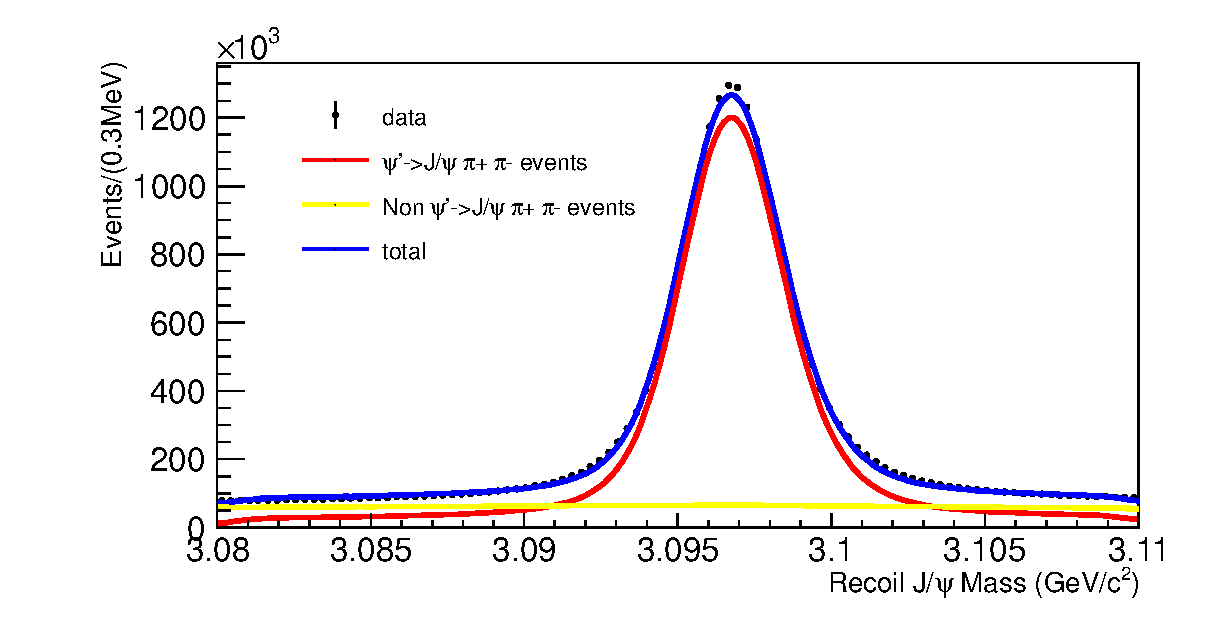
\includegraphics[scale=0.6]{./figure/fitrecoilmass.eps}
\caption{The number of $J/\psi$ events by fitting the recoiling mass of $\pi^+ \pi^-$}
%\label{fig:label}
\end{figure}

\end{paragraph}
\end{subsubsection}
\end{subsection}


\begin{subsection}{Signal and Background}
%\begin{subsection}{common bac}
\begin{paragraph}
\ \ The distributions of $M(\gamma \gamma)_{lg}$ versus $M(\gamma \gamma)_{sm}$ in data and two signal channels are shown in Fig 2,where $M(\gamma \gamma)_{lg}(m_{12})$ and $M(\gamma \gamma)_{sm}(m_{23})$ denote the largest and smallest two-photon invariant mass among three combinations.Three clear vertical bands correspond to three $3 \gamma(J/\psi \to \gamma \eta/\eta'/\pi^0)$ background.These background is suppressed by requiring the invariant mass of any two photons ,$M(\gamma \gamma)$, out of the mass windows [0.10,0.16]$GeV/c^2$,[0.5,0.6]$GeV/c^2$,[0.9,1.0]$GeV/c^2$. The shape of these background which is out of mass window is estimated with high statistic.

\end{paragraph}
\begin{paragraph}
\ \ Before applying mass window cuts, a fit on the distribution of $M(\gamma \gamma)_{sm}$ to determine the yields of $J/\psi \to \gamma \pi^0/\eta/\eta'$ process as shown in Fig.TBD and Table.TBD. The shape of these three channel is retrieved from MC simulation. Their predicted numbers are normalized according to MC efficiencies and their branching fractions are cited in PDG[TBD].


\end{paragraph}
\begin{figure}[!htbp]
\centering
\subfigure[Data]{
\begin{minipage}{5cm}
\centering
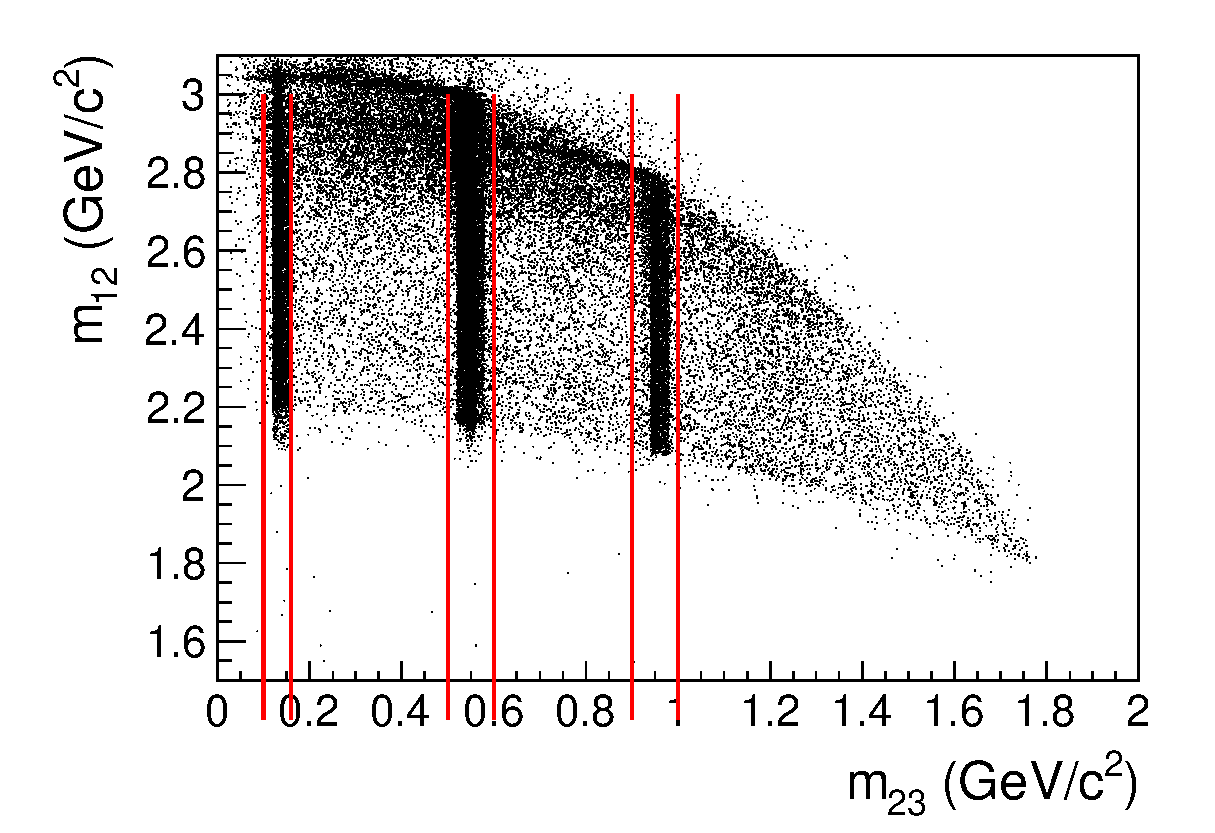
\includegraphics[width=5cm,height = 4cm]{./figure/mass_2D_data.eps}

\end{minipage}

 }
 \centering
\subfigure[3$\gamma$ MC]{
\begin{minipage}{5cm}
\centering
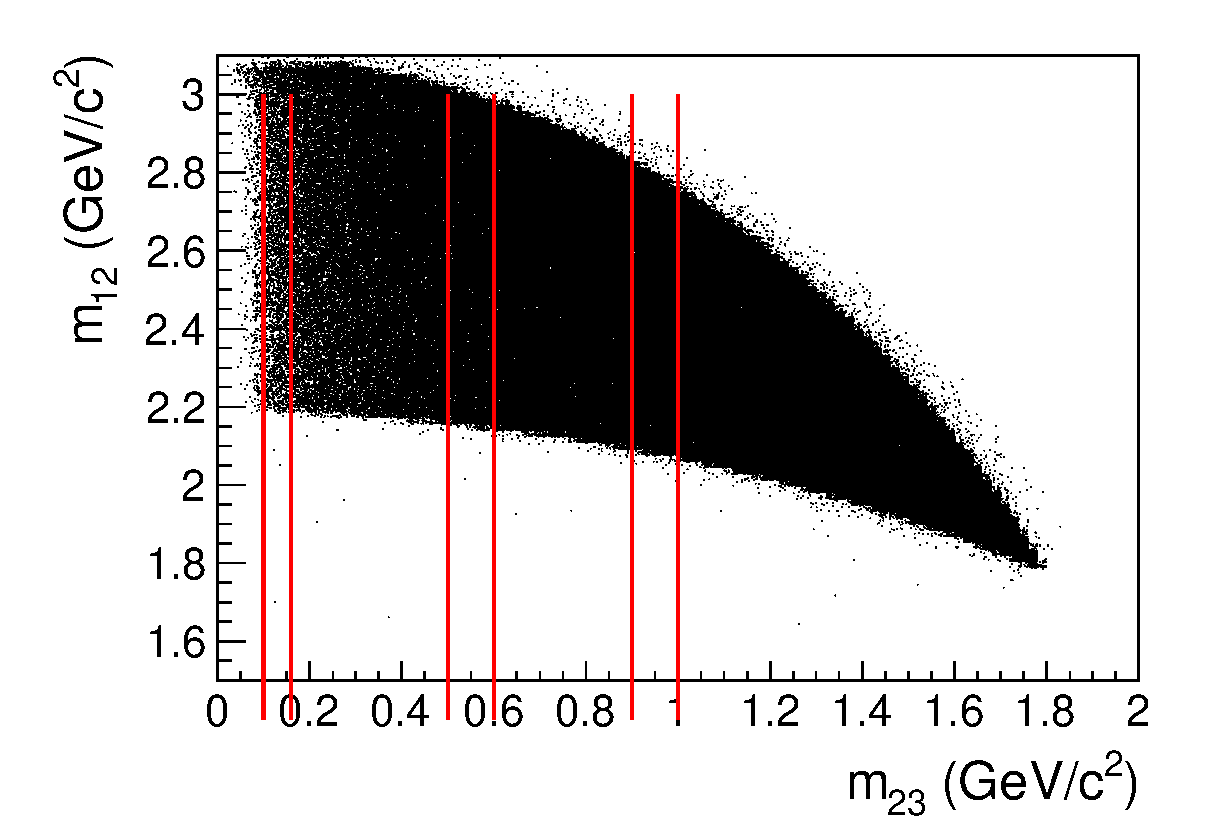
\includegraphics[width=5cm,height = 4cm]{./figure/mass_2D_trin.eps}
\end{minipage}
 }
 \centering
\subfigure[$\gamma \eta_c$ MC]{
\begin{minipage}{5cm}
\centering
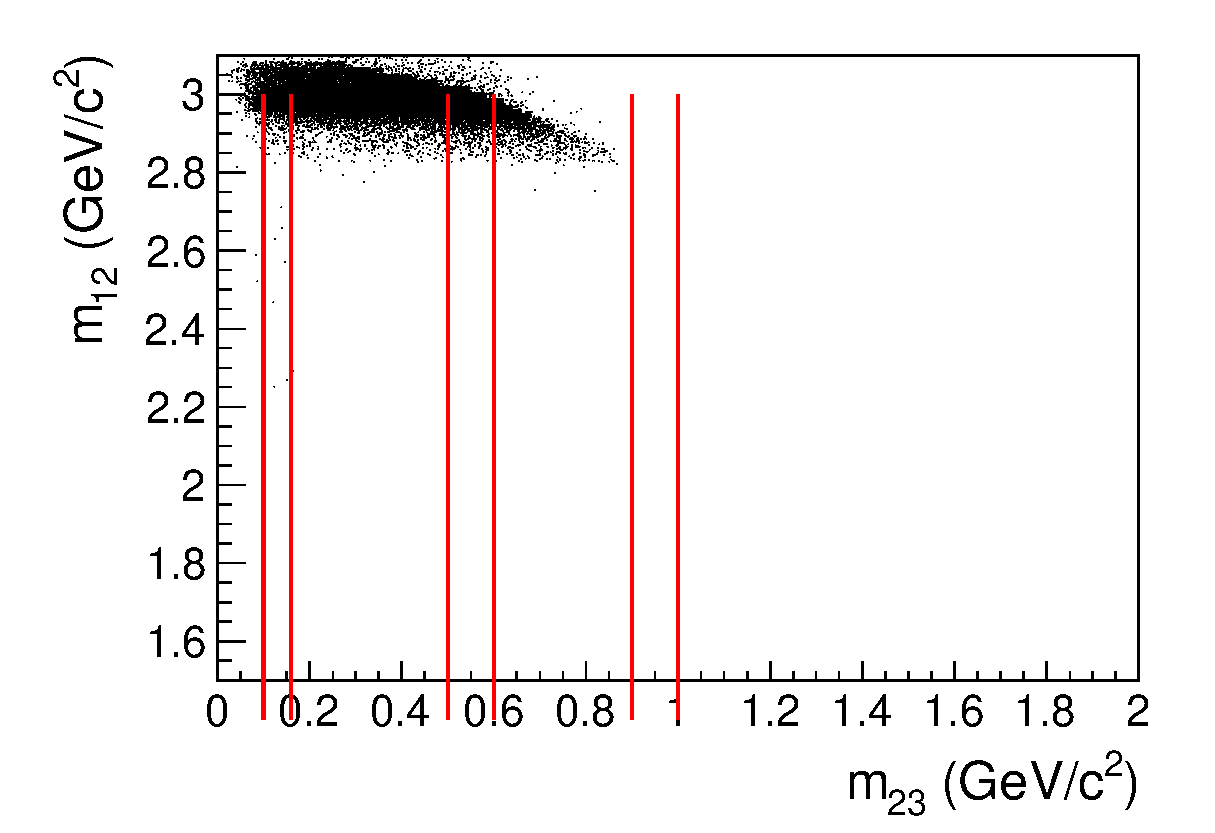
\includegraphics[width=5cm,height = 4cm]{./figure/mass_2D_etc.eps}
\end{minipage}
 }
\caption{Scatter plot of $M(\gamma \gamma)_{lg}$ versus $M(\gamma \gamma)_{sm}$ for data(a) and MC Simulation on the process $J/\psi \to 3\gamma/\gamma \eta_c $ }
%\label{fig:label}
\end{figure}
\begin{figure}[!h]
\centering
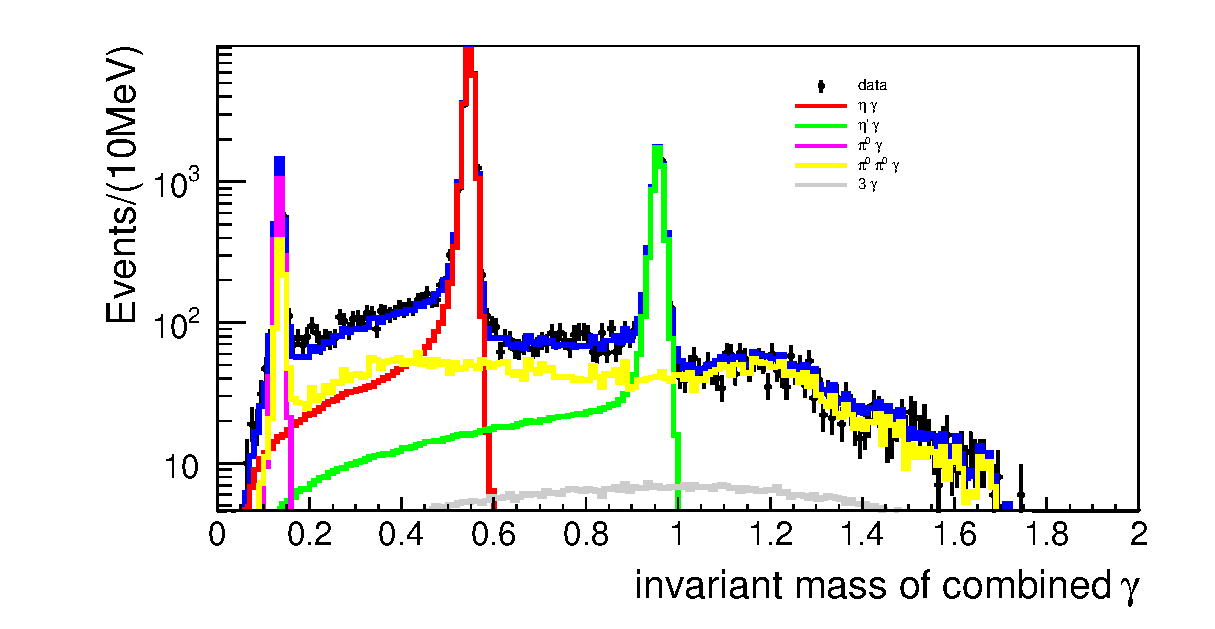
\includegraphics[scale=0.6]{./figure/fitb.eps}
\caption{The log scale plot of fit on $M(\gamma \gamma)_{sm}(m_{23})$}
%\label{fig:label}
\end{figure}

\begin{table}[!h]
  %
  \centering

  \centering
  \begin{tabular}{c|c|c|c|p{3cm}<{\centering}}
  \hline
  Decay channel & Predicted number($N_{J/\psi} \times br$) & Fit number & Efficiencies(\%) & Related branching fraction$(\times 10^{-4})$ \\
  \hline
  $J/\psi \to \gamma (\gamma \gamma)_{\eta}$ & $34935 \pm 1252$ & $ 35859 \pm 248$ & 34.7 & 4.35 \\
  \hline
  $J/\psi \to \gamma (\gamma \gamma)_{\eta'}$ & $9147 \pm 632$ & $ 10318 \pm 152$ & 32.9 & 1.08 \\
  \hline
  $J/\psi \to \gamma (\gamma \gamma)_{\pi^0}$ & $2769 \pm 261$ & $ 2607 \pm 78$ & 37.8 & 0.34 \\
  \hline
  \end{tabular}
   \caption{The fit result on $M(\gamma \gamma)_{sm}(m_{23})$}
  \end{table}

\begin{paragraph}
\ \ In Fig.4, the distributions of the max angle of two photons after applying 3 mass window cuts to $\gamma \eta/\eta'/\pi^0$ MC samples, which is tend to concentrate on the large angle area.So a $\theta_{max} < 165^{\circ}$ cut is applied to select signal events.
\begin{figure}[htbp]
\centering
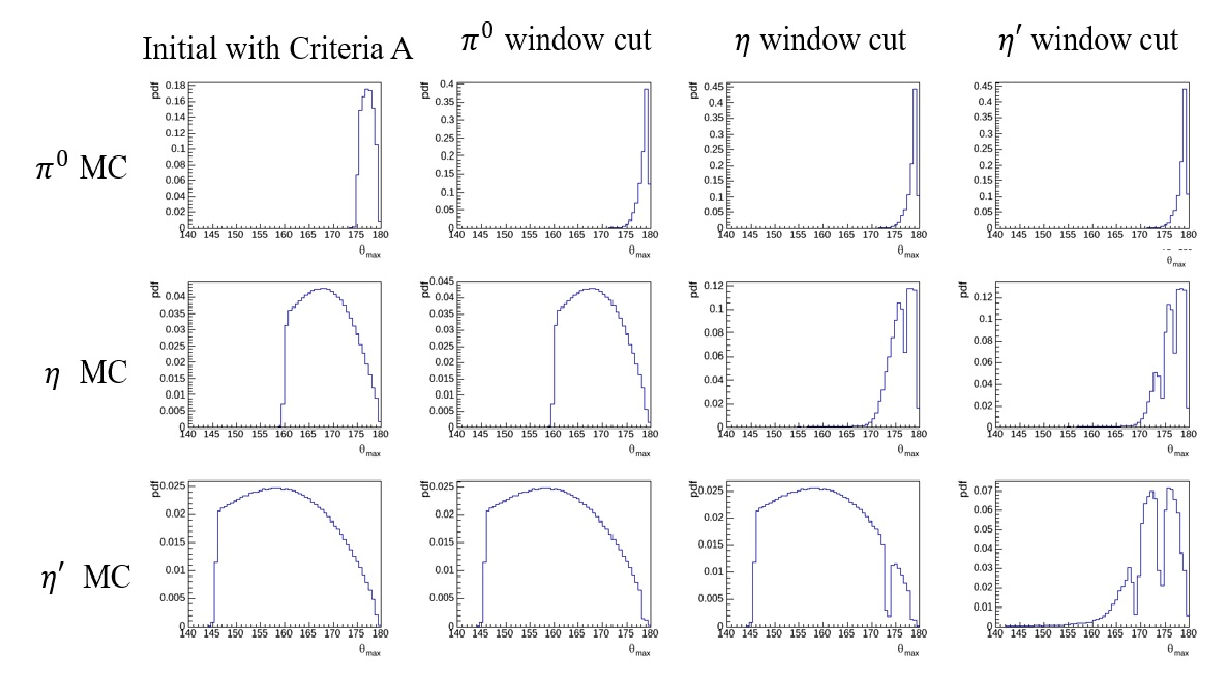
\includegraphics[scale=0.8]{./figure/massjpg.eps}
\caption{The distribution of max angle of two photons after cut Criteria A and three mass window cuts.As shown in the figure,the first column shows the distribution of $J/\psi \to \gamma \pi^0/\eta/\eta'$ MC samples after applying criteria A.The second column shows the same distribution after Criteria A + $\pi^0$ window cut.The third column is after Criteria A + $\pi^0$ +$\eta$ mass window cuts.The last column is after Criteria A + $\pi^0$+$\eta$+$\eta'$.}
%\label{fig:label}
\end{figure}
\end{paragraph}
\begin{paragraph}
\ \ Some events from $J/\psi \to \gamma (\gamma \gamma)_{\pi^0}(\gamma \gamma)_{\pi^0}$ process will pass the selections Criteria A if the two photons from one $\pi^0$ decays are nearly collinear and interpreted as a single cluster,or one of them is very soft.Because large branch ratio of $\gamma \pi^0 \pi^0$ final states,this type of events becomes a primary background after $3\gamma $ background rejection.This type of events consist of numerous intermediate processes.To study this part of backgrounds,one has to disentangle the complicated intermediate resonance.Hence,a partial wave analysis(PWA) was executed in the $J/\psi$ resonant data taken at $\sqrt{s}=3.097GeV$ at the BESIII,following the procedures in the Ref[TBD].
\ \
\end{paragraph}
\begin{paragraph}
\ \ We summarize our selections as below,
\newline \indent  \qquad1.number of charged tracks: $N_{charged-track} = 2$.
  \newline \indent \qquad2.the recoiling mass against $\pi^+ \pi^-$:3.091GeV  $ < M^{\pi^+ \pi^-}_{recoil} < $ 3.103GeV
   \newline \indent  \qquad3.number of photons: $3 \leq N_{photon} \leq 4$.
  \newline \indent \qquad4.$\chi^2_{4C} < 200$,which implies a successful vertex fit
\newline \indent  \qquad5.Mass window cuts.$(0.1,0.16GeV)$ for $\pi^0$,$(0.5,0.6GeV)$ for $\eta$,$(0.9,1.0GeV)$ for $\eta'$.
\newline \indent  \qquad6.The max angle of two photons.$\theta_{max}<165^{\circ}$
\newline \  We group these six cuts as criteria B.The cutflow efficiency table is shown below(Table 3):
\begin{table}[!h]
  %
  \centering

  \centering
  \begin{tabular}{|c|c|c|c|c|c|c|c|}
  \hline
  Sample & \makecell*[c]{MC events\\(data)} & \makecell*[c]{ Events after \\ cut 1-2(eff) }& \makecell*[c] {Events after\\ cut 3-4(eff)} & \makecell*[c] {Events after \\ cut 5(eff)} & \makecell*[c]{Events after \\ cut 6(eff)} & \makecell*[c]{Events after all \\ cuts in data} \\
  \hline
  Data & $\sim$447M & 4296612 & 37420 & 5946 & 2767 & 2767 \\
  \hline
  $J/\psi \to 3\gamma$ & \makecell*[c]{1M\\(1788)} & \makecell*[c]{556918 \\(55.69\%)} & \makecell*[c]{328079\\(32.80\%)}  & \makecell*[c]{267822\\(26.78\%)} &\makecell*[c]{ 196614\\(19.66\%)} & $325 \pm 61 $ \\
  \hline
  $J/\psi \to \gamma \eta$ & \makecell*[c]{10M\\(35859)} &\makecell*[c]{ 5575899 \\(55.75\%) }&\makecell*[c]{3487738\\(34.88\%)} & \makecell*[c]{73978\\(0.739\%)} & \makecell*[c]{272\\(0.0027\%)} & $2.73 \pm 0.01$ \\
  \hline
  $J/\psi \to \gamma \eta'$ & \makecell*[c]{10M\\(10318)} & \makecell*[c]{557064 \\ (55.70\%)} & \makecell*[c]{3289688 \\ (32.89\%)} & \makecell*[c]{63003 \\ (0.63\%)} & \makecell*[c]{4578\\(0.045\%)} & $8.33 \pm 0.01$ \\
  \hline
  $J/\psi \to \gamma \pi^0$ & \makecell*[c]{10M\\(2607)} & \makecell*[c]{5586634\\(55.87\%)} & \makecell*[c]{3779448 \\ (37.79\%)} & \makecell*[c]{64508 \\ (0.646\%)} & 0 & 0 \\
  \hline
  $J/\psi \to \gamma \pi^0 \pi^0$ & 10M & \makecell*[c]{4251832\\(42.51\%)} & \makecell*[c]{210885\\(21.08\%)} & \makecell*[c]{148334 \\ (1.48\%)} & \makecell*[c]{81800 \\ (8.18\%)} & $\sim$ \\
  \hline
  \end{tabular}
   \caption{Cutflow table for Criteria B}
  \end{table}
\end{paragraph}
\begin{paragraph}
\ \ The angle cut will reject almost all the events from $J/\psi \to \gamma \eta_c$(Based on 10M MC generation).So the criteria B is only suitable for the $J/\psi \to 3\gamma$ channel.So a new criteria named as criteria C is grouped as:
\newline \indent  \qquad1.number of charged tracks: $N_{charged-track} = 2$.
  \newline \indent \qquad2.the recoiling mass against $\pi^+ \pi^-$:3.091GeV  $ < M^{\pi^+ \pi^-}_{recoil} < $ 3.103GeV
   \newline \indent  \qquad3.number of photons: $3 \leq N_{photon} \leq 4$.
  \newline \indent \qquad4.$\chi^2_{4C} < 50$,which implies a more strict vertex fit
\newline \indent  \qquad5.Mass window cuts.$(0.1,0.16GeV)$ for $\pi^0$,$(0.5,0.6GeV)$ for $\eta$,$(0.9,1.0GeV)$ for $\eta'$.
%\newline \indent  \qquad6.The max angle of two photons.$\theta_{max}<165^{\circ}$
\newline \ The cutflow efficiency table is shown below(Table 4):
\end{paragraph}
\begin{table}[!h]
  %
  \centering

  \centering
  \begin{tabular}{|c|c|c|c|c|c|c|}
  \hline
  Sample & \makecell*[c]{MC events\\(data)} & \makecell*[c]{ Events after \\ cut 1-2(eff) }& \makecell*[c] {Events after\\ cut 3-4(eff)} & \makecell*[c] {Events after \\ cut 5(eff)}  & \makecell*[c]{Events after all \\ cuts in data} \\
  \hline
  Data & $\sim$447M & 4296612 & 29370 & 2142  & 2142 \\
  \hline
   $J/\psi \to 3\gamma$ & \makecell*[c]{1M\\(1788)} & \makecell*[c]{556918 \\(55.69\%)} & \makecell*[c]{298106\\(29.81\%)}  & \makecell*[c]{243758\\(24.37\%)}  & $435 \pm 87 $ \\
   \hline
   $J/\psi \to \gamma \eta$ & \makecell*[c]{10M\\(35859)} &\makecell*[c]{ 5575899 \\(55.75\%) }&\makecell*[c]{3135402\\(31.35\%)} & \makecell*[c]{36635\\(0.366\%)}  & $235 \pm 1.6$ \\
  \hline
  $J/\psi \to \gamma \eta'$ & \makecell*[c]{10M\\(10318)} & \makecell*[c]{557064 \\ (55.70\%)} & \makecell*[c]{2973855 \\ (29.74\%)} & \makecell*[c]{32390 \\ (0.324\%)}  & $60 \pm 0.9$ \\
  \hline
  $J/\psi \to \gamma \pi^0$ & \makecell*[c]{10M\\(2607)} & \makecell*[c]{5586634\\(55.87\%)} & \makecell*[c]{3386172 \\ (33.86\%)} & \makecell*[c]{36309 \\ (0.363\%)} & $17 \pm 0.5$ \\
  \hline
  $J/\psi \to \gamma \pi^0 \pi^0$ & 10M & \makecell*[c]{4251832\\(42.51\%)} & \makecell*[c]{53418\\(0.534\%)} & \makecell*[c]{39906 \\ (0.399\%)}  & $\sim$ \\
  \hline
  $J/\psi \to \gamma \eta_c$ & 10M(585)& \makecell*[c]{5605041\\(56.05\%)} & \makecell*[c]{2989793\\(29.89\%)} & \makecell*[c]{1926974\\(19.26\%)} & $112 \pm 38$ \\
  \hline

  \end{tabular}
   \caption{Cutflow table for Criteria C}
  \end{table}
%\end{subsection}
%\begin{paragraph}

%\end{paragraph}
\end{subsection}

\begin{subsection}{Analysis}
\begin{subsubsection}{$J/\psi \to 3\gamma$}
\begin{paragraph}
\ \ The kinematic fitting(KF) quality $\chi_{4c}^{2}$ has a good separation power between $3\gamma$ and $\gamma \pi^0 \pi^0$ final states.So in the channel $J/\psi \to 3\gamma$, a 1-D %Some problems
likelihood fitting is implemented on the distribution of KF ($\chi_{4c}^2$) to estimate the signal yield.In the fitting,the shapes of both signal process and background processes are extracted from high statistic MC simulation shown in the last column in Table 3;the numbers of $J/\psi \to \gamma(\gamma \gamma)_{\eta/\eta'/\pi^0}$ are fixed based on MC simulation;the magnitude of $J\psi \to \gamma \pi^0 \pi^0$ process is float.
The fitting result is shown in Fig 4 and Table 5.
 \begin{table}[!b]

  \centering

  \centering
  \begin{tabular}{c|c}
  \hline
   decay channel & $J/\psi \to 3 \gamma$ \\
   \hline
   $\epsilon$(\%) & 35.3\% \\
   yields & $378 \pm 30$ \\
   Branching Ratio($\times 10^{-6}$) & $13.3 \pm 1.0$ \\
   \hline
  \end{tabular}
   \caption{Fitting result for $J/\psi \to 3\gamma$}
  \end{table}
\begin{figure}[!h]
\centering
\subfigure[fit result]{
\begin{minipage}{7cm}
\centering
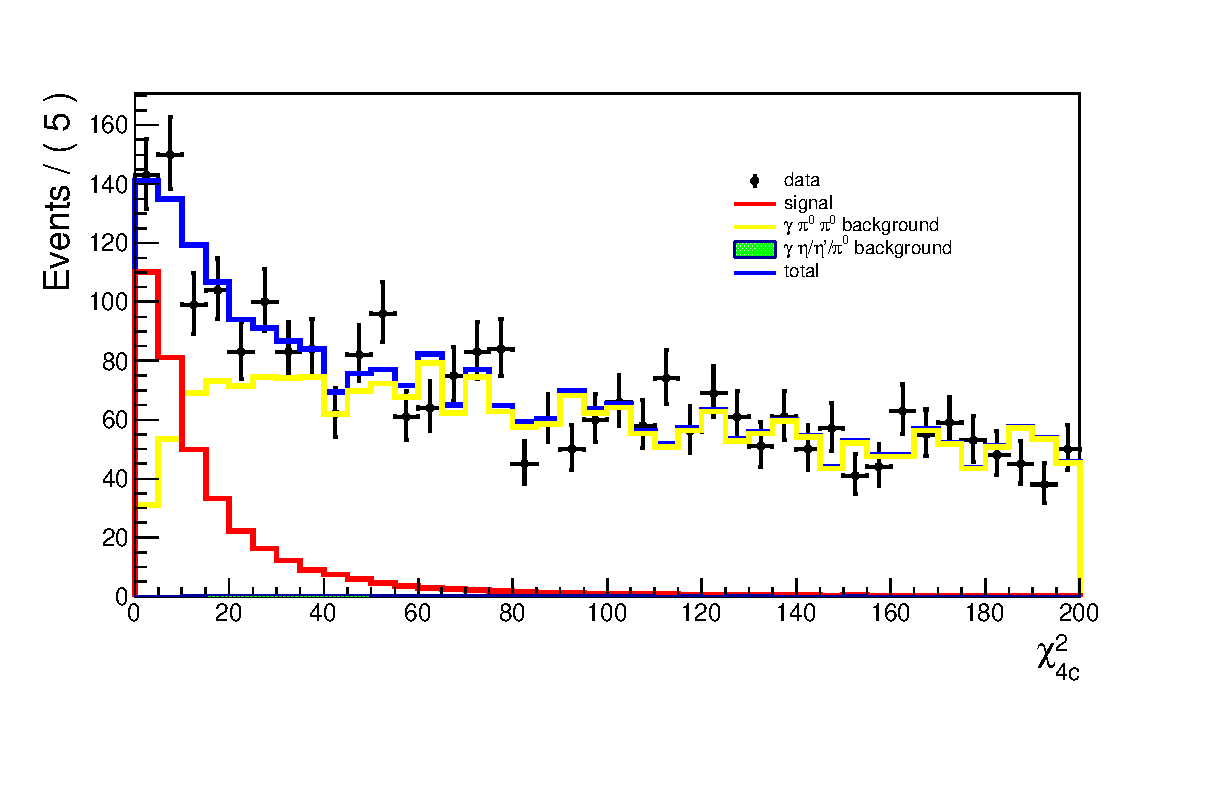
\includegraphics[width=7cm,height = 5.5cm]{./figure/fitchi2_trig.eps}

\end{minipage}

 }
 \centering
\subfigure[fit result in log scale]{
\begin{minipage}{7cm}
\centering
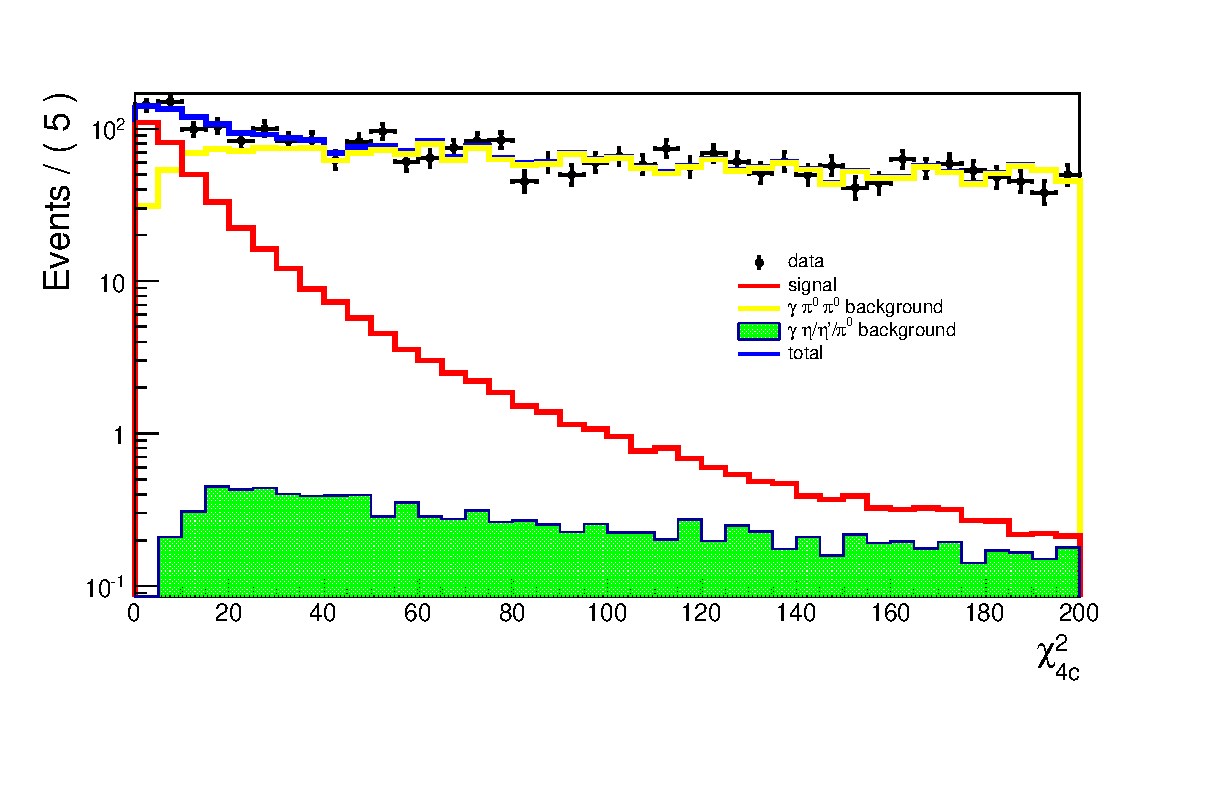
\includegraphics[width=7cm,height = 5.5cm]{./figure/fitchi2_trigLog.eps}
\end{minipage}
 }
 \centering

\caption{$\chi^2_{4c}$ distribution fit result}

%\label{fig:label}
\end{figure}

\end{paragraph}
\end{subsubsection}


\begin{subsubsection}{$J/\psi \to \gamma \eta_c$}
\begin{paragraph}
\ \ The channel $J/\psi \to \gamma \eta_c$ can be distinguished from the distribution of $\chi^2_{4c}$ and distribution of $M(\gamma \gamma)_{lg}$.Therefore,a two-dimensional maximum likelihood fitting is implemented on the these two variables.The projections of the two-dimensional fitting result are shown in Fig.TBD and Table.TBD.In the fitting,the shapes of $J/\psi
\to \gamma (\gamma \gamma)_{\eta/\eta'/\pi^0}$ are fixed based on the MC simulation in Table 4.
\begin{figure}[htbp]
\centering
\subfigure[$\chi^2_{4c}$]{
\begin{minipage}{7cm}
\centering
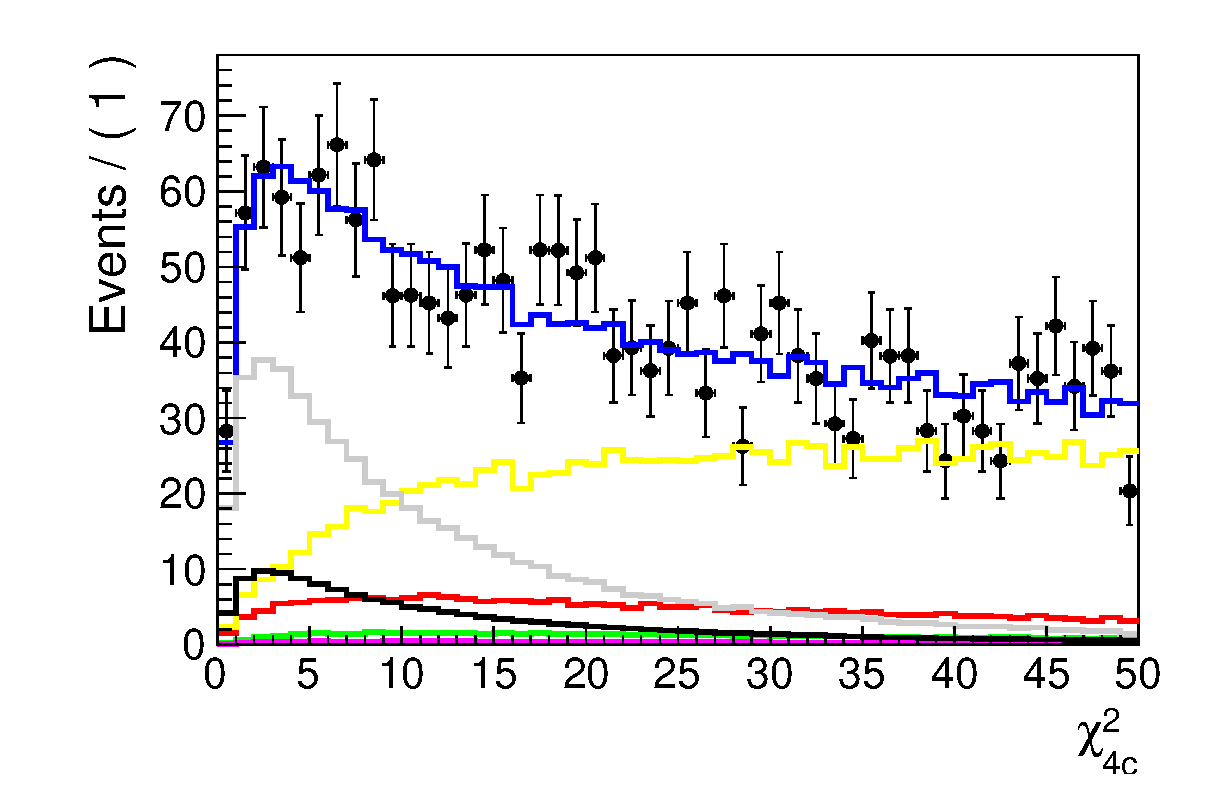
\includegraphics[width=7cm,height = 4cm]{./figure/fit2D_chi2.eps}
\end{minipage}
 }
 \centering
\subfigure[$M(\gamma \gamma)_{lg}$]{
\begin{minipage}{7cm}
\centering
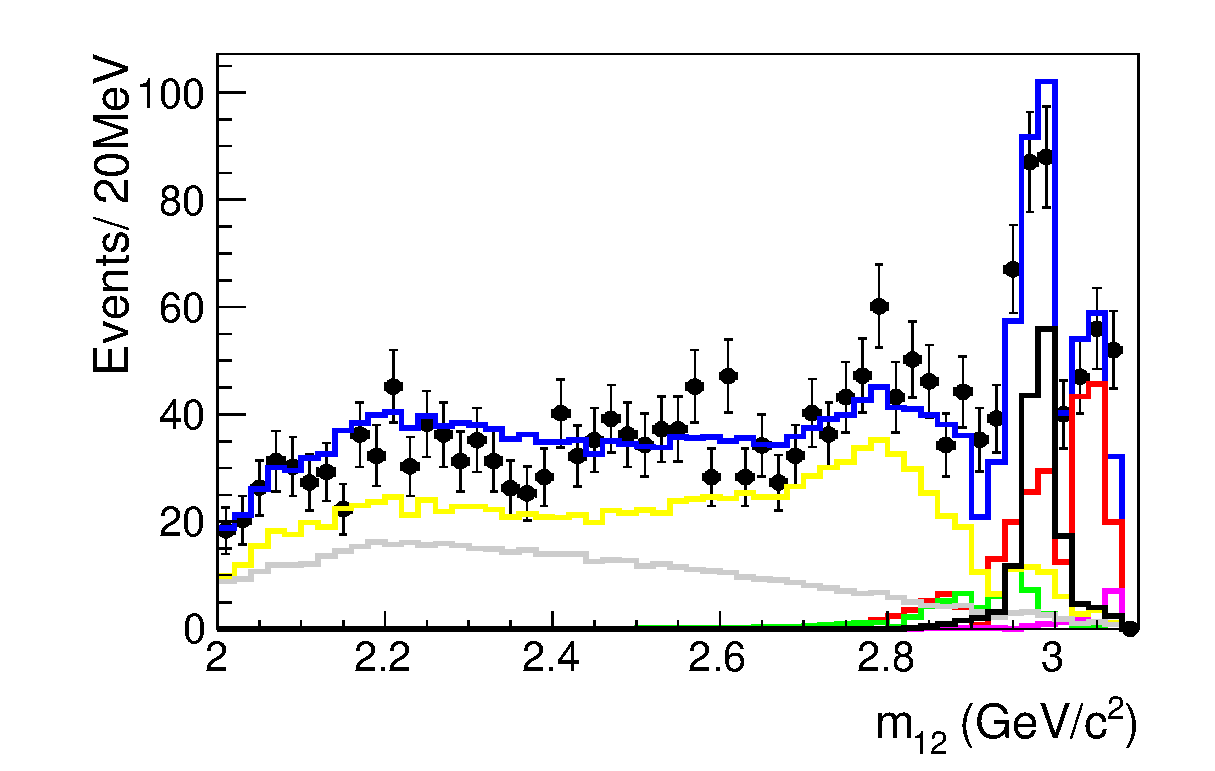
\includegraphics[width=7cm,height = 4cm]{./figure/fit2D_m12.eps}
\end{minipage}
 }
 \centering
\caption{Projection plots of two-dimensional fit to $\chi^2_{4c}$(left) and $M(\gamma \gamma)_{lg}$(right). Here points with error bars are data and the blue line is the sum of the data.The gray line is for process $J/\psi \to 3\gamma$.And the red green purple line are for the channel $J/\psi \to \gamma \eta/\eta'/\pi^0$.The yellow line stands for the distribution of $\gamma \pi^0 \pi^0$}
%\label{fig:label}
\end{figure}
 \begin{table}[!h]
  \centering
  \begin{tabular}{c|c|c}
  \hline
   decay channel & $J/\psi \to 3\gamma $ & $J/\psi \to \gamma \eta_c$\\
   \hline
   $\epsilon$(\%) & 43.8\% & 34.4\% \\
   yields & $519 \pm 36$ & $146 \pm 17$\\
   Branching Ratio($\times 10^{-6}$) & $14.7 \pm 1.0$ & $5.3 \pm 0.6$ \\
   \hline
  \end{tabular}
   \caption{Fitting result for two-dimensional likelihood fit}
  \end{table}
\end{paragraph}
\end{subsubsection}
\end{subsection}

\bigskip
\begin{subsection}{Study on $\eta_c$ shapes}
\begin{paragraph}
\ \ A study on the $\eta_c$'s shape based on result of two-dimensional likelihood fit.With removal of all the background based on the fit result,formula $F_{\eta_c} = \sigma \otimes (BW(m) \times E_{\gamma}^3 \times \varepsilon(m) \times f_{dump})$ is applied to fit the invariant mass of $\eta_c$.The $\sigma$ is the resolution function of the detector. And the convolution includes three parts:Breit-Wigner function,the energy of radiative photon and dumping factor.The dumping factor is expressed as $f_{dump} = \frac{E_0^2}{E_0 \times E_{\gamma} + (E_0 - E_{\gamma})^2}$.Figure TBD shows the result. A first-order polynomial is utilized to estimate the non-physical background.The fitting result is shown in Table TBD.
\begin{figure}[!h]
\centering
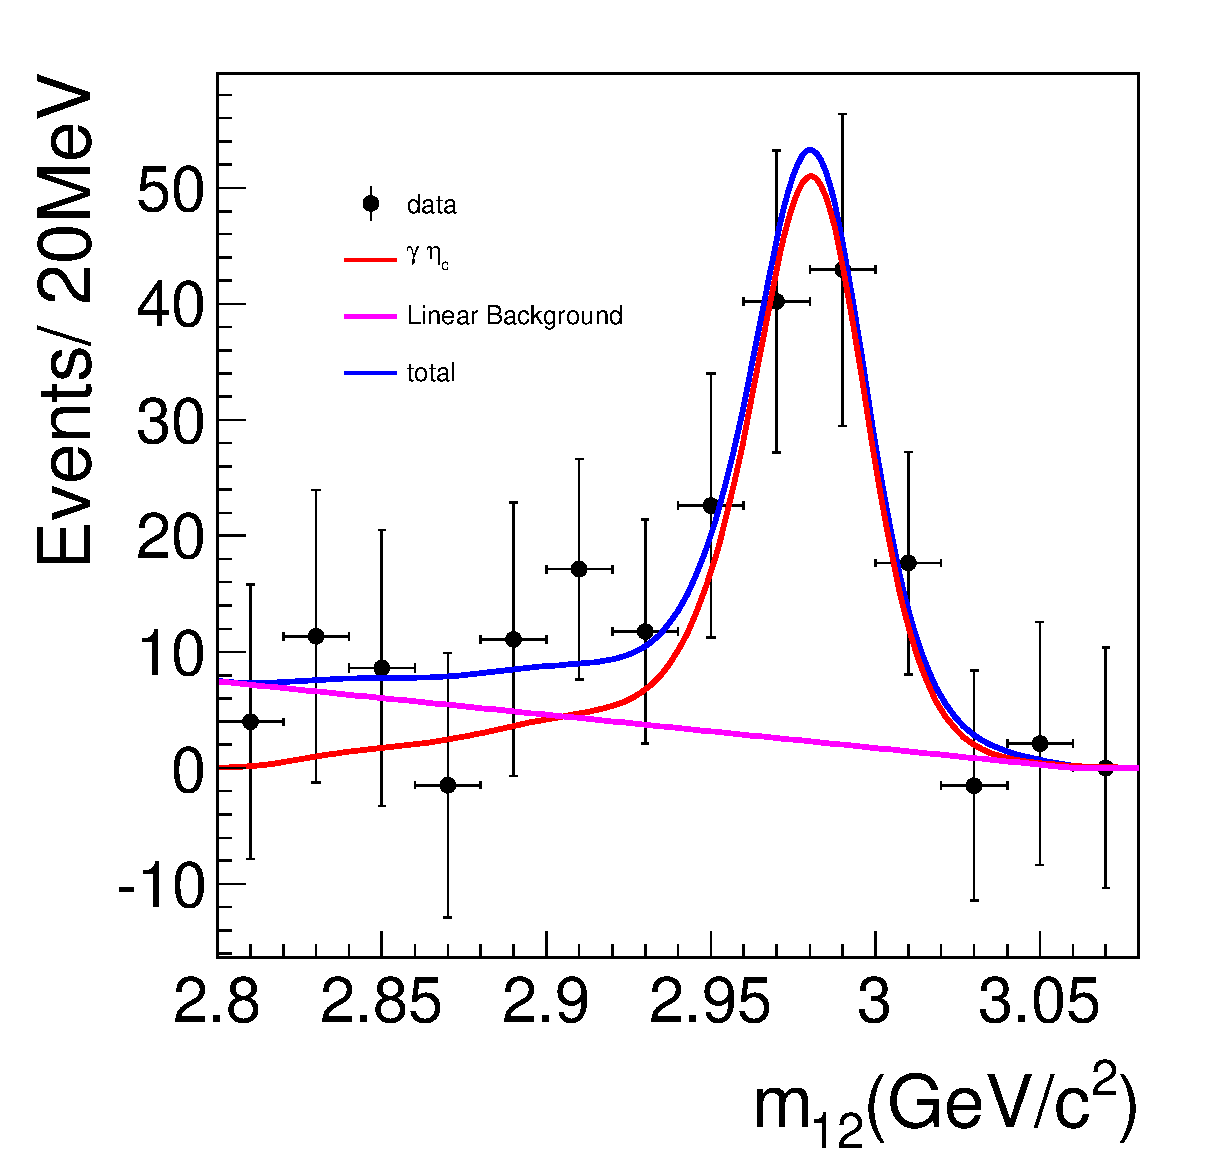
\includegraphics[width=7cm,height = 5cm]{./figure/etc_fit.eps}
\caption{$\eta_c$ shape}
\end{figure}
 \begin{table}[!h]
  \centering
  \begin{tabular}{c|c}
  \hline
   decay channel & $J/\psi \to \gamma \eta_c$ \\
   \hline
   $\epsilon$(\%)  & 34.4\% \\
   yields  & $138 \pm 13$\\
   Branching Ratio($\times 10^{-6}$) & $5.0 \pm 0.5$ \\
   \hline
  \end{tabular}
   \caption{Fit result for lineshape fit}
  \end{table}
\end{paragraph}
\begin{paragraph}
\newline
\ \ A study of a interference between $J/\psi \to \gamma \eta_c$ and $J/\psi \to 3\gamma$ is considered.Based on two-dimensional fit result, the backgrounds except for process $J/\psi \to 3\gamma$ and $J/\psi \to \gamma \eta_c$ are removed for analyzing these two channel's interference. The formula $F_{inter} = \sigma \otimes (|\alpha \times e^{i\phi} \times BW_{\eta_c}(m) \times \sqrt{f_{dump} }+ f_{3\gamma}|^2 \times E_{\gamma} \times \varepsilon(m))$ is applied to study this phenomenon.The $\sigma$ ,$\varepsilon$ or $E_{\gamma}$ is as demonstrated in the last paragraph.And the $\phi$  and $\alpha$ are the interference angle and interference relative strength separately.Figure TBD shows the result.And a interference angle likelihood scan is also manipulated to calculated the significance of this phenomenon.So the significance of this phenomenon is about $1.5\sigma$.

\begin{figure}[!h]
\centering
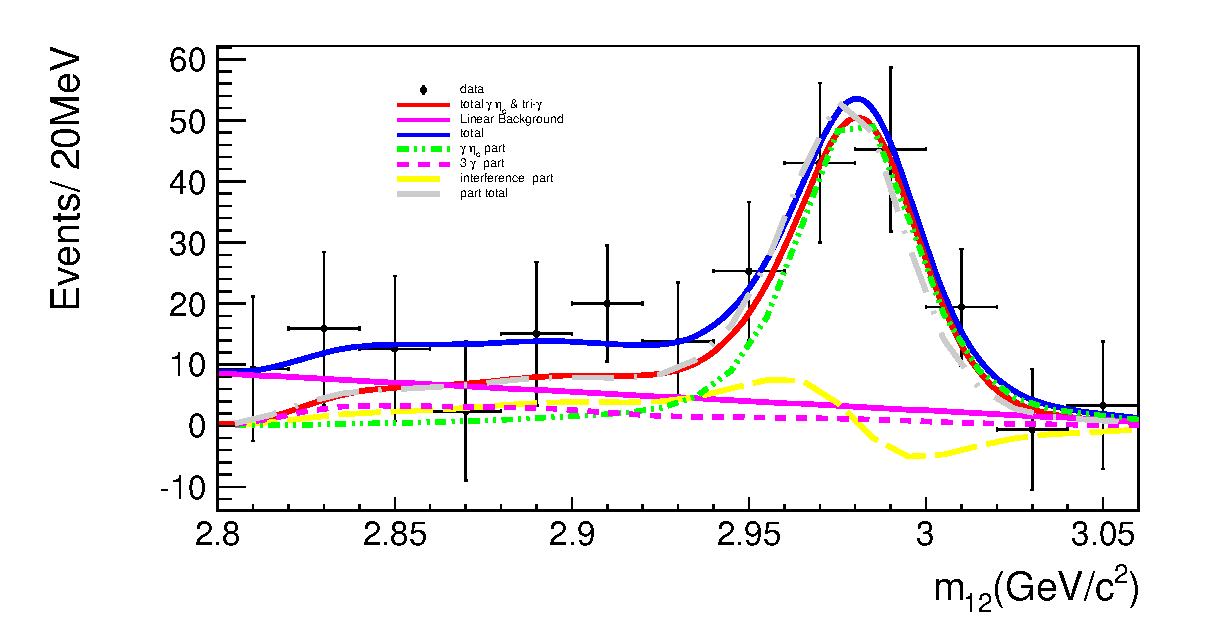
\includegraphics[width=11cm,height = 7cm]{./figure/inter_part.eps}
\caption{interference study}
\end{figure}
\begin{figure}[!ht]
\centering
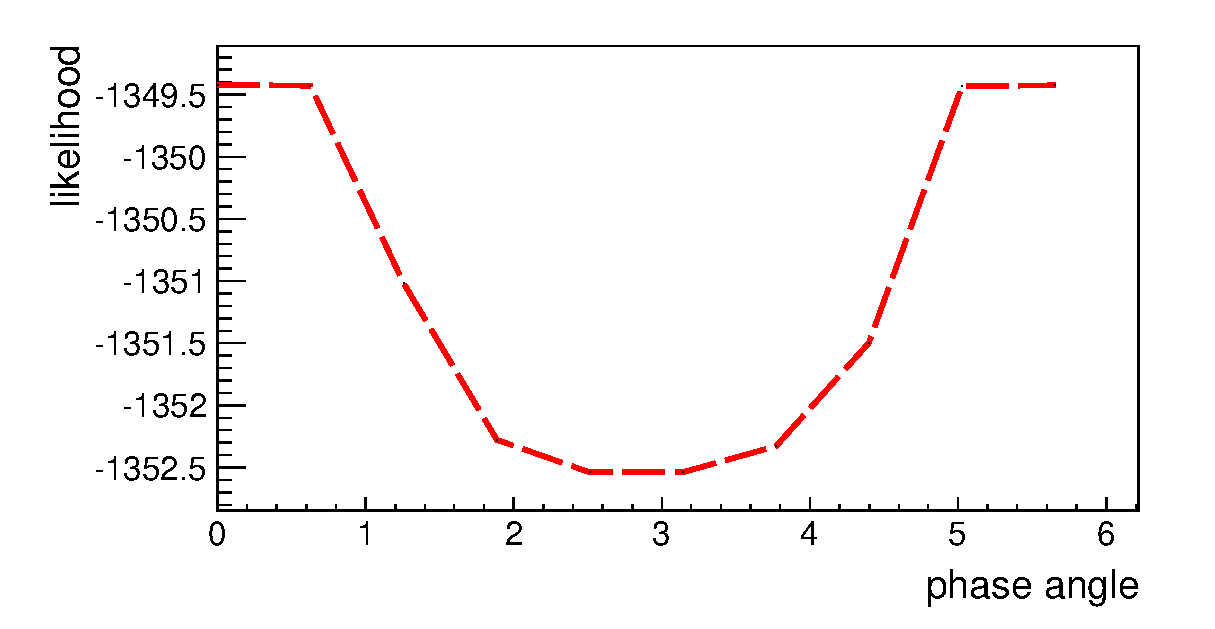
\includegraphics[width=8cm,height = 4.5cm]{./figure/likelihood_scan.eps}
\caption{likelihood scan}

\end{figure}
\begin{table}[!h]
  \centering
  \begin{tabular}{c|c}
  \hline
   Parameters & Value \\
   \hline
   $\sigma(MeV)$ & 9.9 \\
   \hline
   $\phi$ & 3.16 \\
   \hline
   $\alpha$ & 3.63 \\
   \hline
  \end{tabular}
   \caption{Interface parameters}
  \end{table}
\end{paragraph}
\end{subsection}

\begin{subsection}{Systematic Errors}
\begin{paragraph}
 \ \ Systematic errors study is based on former study and listed in the Table TBD.In our study,the matrix elements item
 is estimated by fitting the data in different bin varying by different energy and polar angle.
 \begin{table}[!h]
  \centering
  \begin{tabular}{|c|c|c|}
  \hline
   \multirow{2}{*}{Sources} & \multicolumn{2}{ |c| }{relative uncertainties(\%)} \\
   \cline{2-3}
   & $J/\psi \to 3 \gamma$ & $J/\psi \to \gamma \eta_c$ \\
   \hline
   photon detection & 1.6 & 1.6 \\
   \hline
   Number of good photons & 0.5 & 0.5 \\
   \hline
   KF and $\chi^2_{4c}$ requirement & 2 & 2 \\
   \hline
   PWA model & 2 & 2 \\
   \hline
   $\eta/\eta'/\pi^0$ rejection & 0.5 & 5 \\
   \hline
   Number of $J/\psi$ & $<0.1$ & $<0.1$ \\
   \hline
   Matrix elements & 6 & $-$ \\
   \hline
   Fitting and photon angle rejection & 6 & 6\\
   \hline
   total & 9 & 6.8 \\
   \hline

  \end{tabular}
   \caption{Summary of the systematic uncertainties. $'-'$ means negligible}
  \end{table}
 \end{paragraph}
\end{subsection}


\end{section}

\clearpage
\begin{section}{Conclusion}
\begin{paragraph}
\ \ By analyzing the $\psi(2s)$ data taken at $\sqrt{s} = 3.686GeV$ using $\psi(2s) \to \pi^+ \pi^- J/\psi$ with BESIII detector at the BEPCII collider during 2009 and 2012,measurements on the branching ratio of process $J/\psi \to 3\gamma$ and $J/\psi \to \gamma \eta_c \to \gamma (\gamma \gamma)_{\eta_c}$ are demonstrated as:$\mathcal{B}_{J/\psi \to 3\gamma} = 13.3 \pm 1.0 \pm 1.2$
, and $\mathcal{B}_{J/\psi \to \gamma \eta_c \to \gamma (\gamma \gamma)_{\eta_c}} = 5.3 \pm 0.6 \pm 0.4$.

\end{paragraph}


\end{section}

\clearpage
%%%%%%%%%%%%%%%%%%%%%%%%%%%%%%%%%%%%%%%%%%%%%%%%%%%%%%%%%%%%%%%%%%%%%%%%%%%%%%%
%\appendix
%\part*{Appendices}
%%\addcontentsline{toc}{part}{Appendices}
%\include{Appendix_vrcut}


%%\include{10Summary}
%
%%%%%%%%%%%%%%%%%%%%%%%%%%%%%%%%%%%%%%%%%%%%%%%%%%%%%%%%%%%%%%%%%%%%%%%%%%%%%%%
%%%=============================================================================
%\clearpage
%
%\bibliographystyle{besnote}
%%\bibliography{Lambdac4600}
%\include{bibite}
\addcontentsline{toc}{section}{References}
\begin{thebibliography}{99}
%\bibitem{pub:current} J.D. Bjorken and S.D. Drell, Relativistic Quantum Mechanics,  McGraw-Hill, New York, 1964.
%\bibitem{pub:coulombcorr} A. B. Arbuzov, T. V. Kopylova, JHEP 1204, 009 (2012);
%\bibitem{SM1967}S.Weinberg, Phys. Rev. Lett. {\bf 19}, 1264(1967)
%\bibitem{pub:exp1} L. Andivahis et al., Phys. Rev. D50, 5491 (1994).
%\bibitem{pub:exp2} M.K. Jones et al., Phys. Rev. Lett. 84, 1398 (2000).
%\bibitem{pub:exp3} O. Gayou et al., Phys. Rev. Lett. 88, 092301 (2002).
%\bibitem{pub:exp4} M. Castellano et al., Nuovo Cimento 14, 1 (1973).
%\bibitem{pub:exp5} M. Ambrogiani et al., Phys. Rev. D60, 032002 (1999).
%\bibitem{pub:exp6} A. Antonelli et al., Nucl. Phys. B517, 3 (1998).
%\bibitem{pub:exp7} J. P. Lees et al. (BABAR Collaboration), Phys. Rev. D 88, 072009 (2013).
%\bibitem{pub:exp8} G. Bardin et al. (PS170 Collaboration), Nucl. Phys. B411, 3(1994).
%\bibitem{pub:exp9} A. Antonelli et al, (FENICE Collaboration), Nucl. Phys. B517,3(1998).
%\bibitem{pub:exp10} 10th International Workshop on $e^+e^-$ collisions from $\phi$ to $\psi$ (PhiPsi15).
%\bibitem{pub:bes3} M. Ablikim et al. [BESIII Collaboration], Nucl. Instrum. Meth. A 614, 345 (2010).
%\bibitem{pub:boss1} S. Agostinelli et al. [GEANT Collaboration], Nucl. Instrum. Meth. A 506, 250 (2003); J. Allison et al., IEEE Trans. Nucl. Sci. 53, 270 (2006).
%\bibitem{pub:boss2} Z. Y. Deng et al., High Energy Physics and Nuclear Physics 30, 371 (2006).
% [8] F. Iachello, A.D. Jackson and A. Lande, Phys. Lett. 43B,  191 (1973).
%  [9] J. Ashman et al., Nucl. Phys. B328, 1 (1989).
%  [10] G. Holzwarth, Z. Phys. A356, 339 (1996).
%   [11] M.R. Frank, B.J. Jennings, and G.A. Miller, Phys. Rev. C54,  920 (1996).
%   [12] F. Cardarelli and S. Simula, Phys. Rev. C62, 065201 (2000).
\end{thebibliography}






\end{document}
%%%%%%%%%%%%%%%%%%%%%%%%%%%%%%%%%%%%%%%%%%%%%%%%%%%%%%%%%%%%%%%%%%%%%%%%%%%%%%

